\fancyhead{}
\fancyfoot{}
\cfoot{\thepage}

\lhead{Resultados}

\chapter{Resultados}

\section{Métricas de rendimiento}
Las métricas de rendimiento son medidas cuantitativas utilizadas en aprendizaje automático para evaluar la calidad de los modelos predictivos. Estas métricas proporcionan una evaluación objetiva de la capacidad de un modelo para hacer predicciones precisas en tareas como clasificación o regresión. 
\subsection{Modelo de regresión lineal}

los parámetros y configuraciones utilizados en el modelo de regresión con regularización Ridge:

\begin{itemize}
  \item  \textbf{loss=squared\_loss:} Se ha elegido la función de pérdida de error cuadrático medio (MSE) debido a la naturaleza de un problema de regresión. La función MSE evalúa la discrepancia al cuadrado entre las predicciones y los valores reales, y se minimiza durante el proceso de entrenamiento.

    
  \item \textbf{penalty=l2:} La regularización Ridge ayuda a prevenir el sobreajuste incorporando un término de penalización en la función de pérdida.

  
  \item \textbf{alpha=0.0001:}  En este caso, se ha optado por un valor pequeño (0.0001) para evitar una regularización excesiva y permitir que el modelo se ajuste de manera adecuada a los datos.

  
  \item \textbf{max\_iter=1000:} Se ha establecido el número máximo de iteraciones permitidas para el descenso de gradiente en 1000, un valor suficientemente amplio para asegurar la convergencia del modelo.

  
  \item \textbf{tol=1e-3:} Este valor de tolerancia es apropiado para garantizar una convergencia razonable.

  
  \item \textbf{learning\_rate=constant:} Se ha configurado la tasa de aprendizaje como constante a lo largo del proceso de entrenamiento.
\end{itemize}
   
 

  \begin{figure}[H]
    \begin{center}
      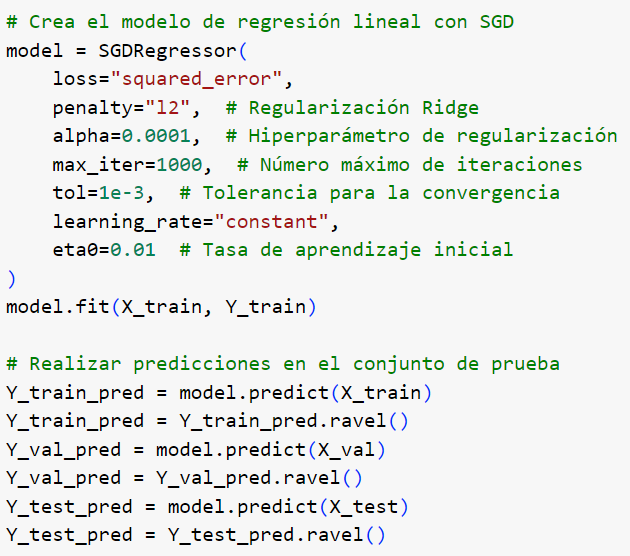
\includegraphics[scale=0.50]{./regresion lineal estructura.png}
      \caption{Algoritmo de la estructura de regresión lineal.}
      \label{fig:estructura_lineal}
    \end{center}
  \end{figure}

  
A pesar de que tanto el Error Cuadrático Medio (MSE) como el Error Absoluto
Medio (MAE) proporcionan indicadores favorables, el valor de R-cuadrado (R²)
indica que el modelo se encuentra notablemente alejado de la excelencia
representada por un valor de 1, ya que R² = 1 constituye la condición ideal
(Figura \ref{fig:metricas_regresion}).

\begin{figure}[H]
  \begin{center}
    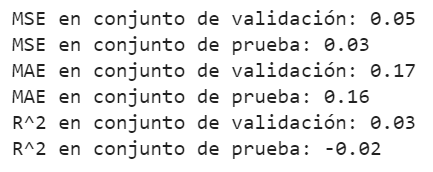
\includegraphics[scale=0.70]{./metricas de error REGRESION LINEAL.png}
    \caption{Metrica de error regresión lineal.}
    \label{fig:metricas_regresion}
  \end{center}
\end{figure}

% \begin{figure}[H]
%   \begin{center}
%     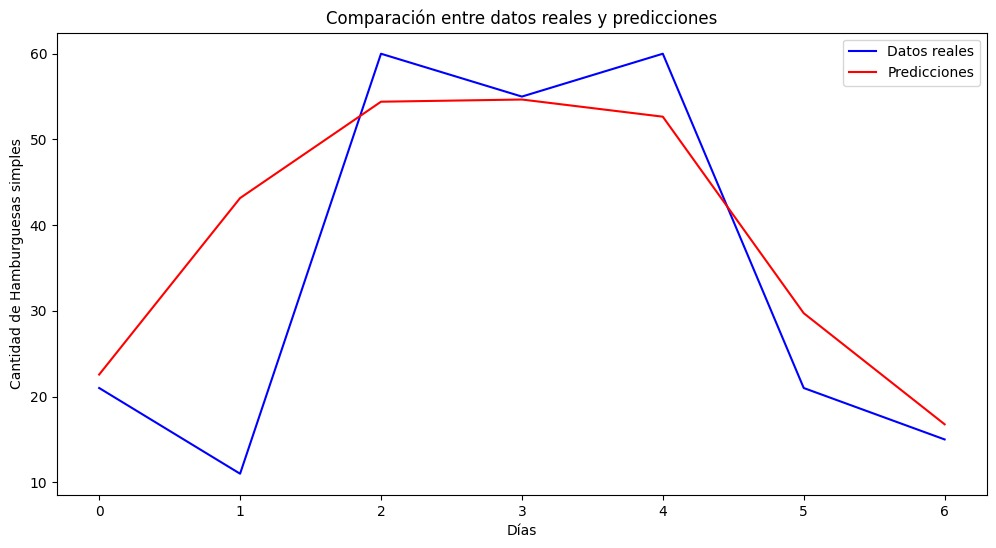
\includegraphics[scale=0.50]{./modeloLineal7Dias.jpg}
%     \caption{Predicción de 7 días con regresión lineal.}
%     \label{fig:grafico_lstm}
%   \end{center}
% \end{figure}

\subsection{Modelo LSTM}

% \begin{figure}[H]
%   \begin{center}
%     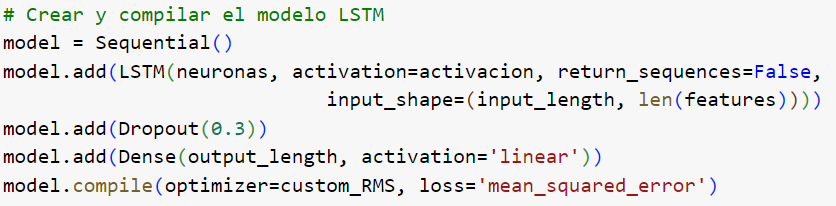
\includegraphics[scale=0.60]{./arquitectura LSTM.png}
%     \caption{Algoritmo de la estructura del LSTM.}
%     \label{fig:estructura_lstm}
%   \end{center}
% \end{figure}

Al configurar una red neuronal LSTM, es común considerar varios hiperparámetros
clave (Codigo \ref{fig:codigo_lstm}):

\begin{itemize}
  \item  \textbf{Unidades de LSTM:} Se obtuvieron los mejores resultados con 64 neuronas.
   
  
  \item \textbf{Número de capas LSTM:} En este caso, se determinó que una sola capa oculta era la mejor opción.

 
  \item \textbf{Función de Activación:} Se lograron buenos resultados utilizando “relu” en la capa oculta y “linear” en la salida.

 
  \item \textbf{Función de Pérdida:} Se optó por el MSE debido a su versatilidad en problemas de regresión.

 
  \item \textbf{Optimizador:} En esta configuración, se prefirió “RMSprop” por su relevancia en predicciones de demanda.

 
  \item \textbf{Tasa de Aprendizaje:} Una tasa de aprendizaje de 0.01 resultó óptima.

 
  \item \textbf{Dropout:} Para esta configuración, un dropout del 20\% fue suficiente.
\end{itemize}

\begin{figure}[H]
  \begin{center}
    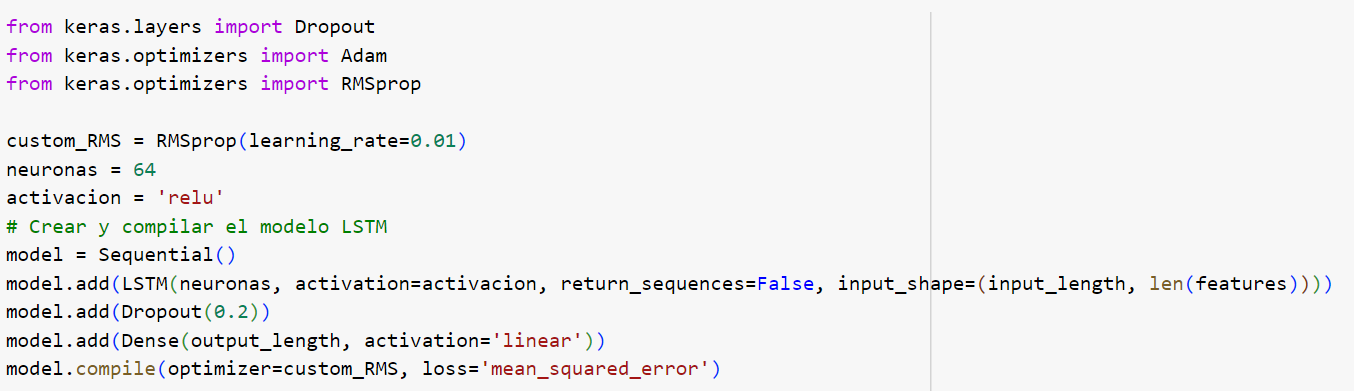
\includegraphics[scale=0.40]{./LSTM estructura.png}
    \caption{Algoritmo de estructura LSTM.}
    \label{fig:codigo_lstm}
  \end{center}
\end{figure}

% Es importante tener en cuenta que la elección de estos hiperparámetros puede depender en gran medida del problema específico y requiere experimentación para encontrar la configuración óptima.

\begin{figure}[H]
  \begin{center}
    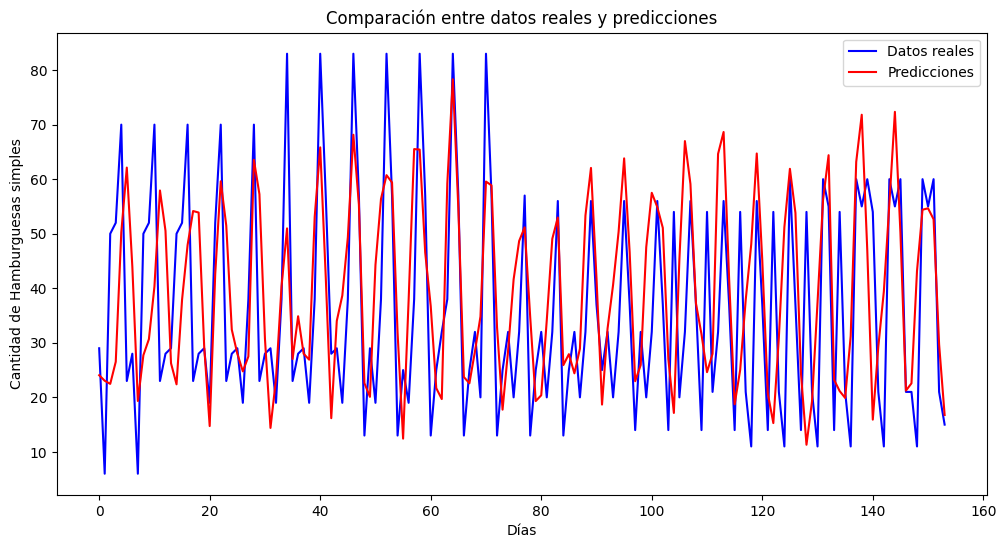
\includegraphics[scale=0.50]{./predicción 7 días.png}
    \caption{Grafico de predicción con LSTM.}
    \label{fig:grafico_lstm}
  \end{center}
\end{figure}

Los tres valores muestran una proximidad aceptable, lo que indica que el modelo
tiene una capacidad de generalización satisfactoria (Figura
\ref{fig:desenpeño}).
\begin{figure}[H]
  \begin{center}
    \includegraphics[scale=0.50]{./comparativo desempeños LSTM.png}
    \caption{Comparativo de desempeños LSTM.}
    \label{fig:desenpeño}
  \end{center}
\end{figure}

En este trabajo para evaluar el rendimiento de una red neuronal LSTM se hace uso de la función de pérdidas (loss). Esta permite evaluar cómo es su evolución
de los datos en un modelo. Según la literatura entre más grandes las pérdidas
las predicciones van a estar alejadas del valor real. En la (Figura
\ref{fig:perdida}) se puede observar la evolución de pérdidas a través de las
épocas, se evidencia dos señales que corresponden a entrenamiento y validación
marcados con los colores azul y naranja respectivamente, se infiere que los
valores decrecen con una alta tasa hasta la época 5 aproximadamente y luego no
presentan cambios significativos. Las pérdidas son de 0.020 y 0.039 para
entrenamiento y test respectivamente.

\begin{figure}[H]
  \begin{center}
    \includegraphics[scale=0.50]{./grafico de perdida en las épocas.png}
    \caption{Grafico de perdida en las épocas LSTM.}
    \label{fig:perdida}
  \end{center}
\end{figure}
\section{Resultados de predicción de compras}

\begin{table}[H]
  \centering
  \begin{tabular}{|c|c|c|c|c|c|}
    \hline
    \rowcolor{gray!50} \textbf{Días} & \textbf{Real} & \textbf{Pred. Reg} & \textbf{Dif} & \textbf{Pred. LSTM} & \textbf{Dif} \\
    \hline
    1 & 21 & 39 & 18 & 33 & 12 \\
    \hline
    2 & 11 & 42 & 31 & 41 & 30 \\
    \hline
    3 & 60 & 44 & -16 & 52 & -8 \\
    \hline
    4 & 55 & 47 & -8 & 47 & -8 \\
    \hline
    5 & 60 & 34 & -26 & 36 & -24 \\
    \hline
    6 & 21 & 36 & 15 & 22 & 1 \\
    \hline
    7 & 15 & 39 & 24 & 27 & 12 \\
    \hline
    Dif. Total &  &  & 38 &  & 15 \\
    \hline
  \end{tabular}
  \caption{ Tabla de resultados de las predicciones de ambos modelos}
  \label{tab:prediccion_final}
\end{table}

La tabla~\ref{tab:prediccion_final} proporciona un resumen de la predicción de la demanda de productos de la empresa gastronómica durante un período de siete días. 

\vspace{1\baselineskip}
Compara los resultados entre los modelos de predicción estudiados: el modelo de regresión lineal y el modelo LSTM (Long Short-Term Memory).

\vspace{1\baselineskip}
En la columna  “Días”, se enumeran los siete días del período en cuestión. En  “Real”, se muestra la demanda real de productos para cada día, mientras que en “Pred. Reg” y “Pred. LSTM”, se presentan las predicciones realizadas por los modelos de regresión lineal y LSTM, respectivamente.

\vspace{1\baselineskip}
La columna “Dif” representa la diferencia entre las predicciones de cada modelo y la demanda real. En términos generales, se puede observar que ambas técnicas tuvieron algunas discrepancias con los valores reales. El modelo de regresión lineal tuvo una diferencia total de 38 unidades en comparación con la demanda real, mientras que el modelo LSTM tuvo una diferencia total de 15 unidades. En este caso, el modelo LSTM muestra un mejor desempeño al ser más preciso en la predicción de la demanda de productos en estos siete días en comparación con el modelo de regresión lineal.

\vspace{1\baselineskip}
En resumen, este estudio ha avanzado significativamente en la solución del problema de la predicción de la demanda semanal, y se espera que futuras investigaciones sigan ampliando los límites de la precisión y la aplicabilidad de estas predicciones en entornos de demanda.



% Este captulo presenta el producto del anlisis de los datos. Los resultados compendian el eventual tratamiento estadstico que se dio a los datos. Regularmente el orden es: a) anlisis descriptivo de los datos, b) anlisis inferenciales para responder a las preguntas de investigacin y/o probar hiptesis. Segn \cite{sampieri}, la American Psychological Association recomienda que primero se describa de manera breve la idea principal que resume los descubrimientos, y posteriormente se los reporten con detalle. Es importante destacar que en este captulo no se incluyen conclusiones ni sugerencias, tampoco se deben explicar las implicaciones de la investigacin. Esto se hace en el captulo dedicado a la interpretaciones de los resultados, que en esta plantilla se denomina ``Discusin''.

% Aqu el investigador se limita a describir sus hallazgos. Una manera til de hacerlo es mediante elementos como tablas, grficas, dibujos, diagramas, mapas y figuras generados por el anlisis. Son elementos que sirven para organizar datos, de tal manera que el lector los pueda leer y entender las los vnculos entre las variables. Cada uno de dichos elementos debe ir enumerado. Una buena regla para elaborar una tabla es organizarla lgicamente y eliminar la informacin que pudiera confundir al lector.

% Es conveniente brindar una sencilla explicacin de las pruebas realizadas y presentar los resultados de la manera ms comprensible posible. En este caso las tablas deben ser descritas. Los diagramas, figuras, mapas cognoscitivos, esquemas, matrices y otros elementos grficos tambin deben ser numerados segn una  lgica secuencial. Se debe observar el principio bsico: una buena figura es sencilla, clara y no estorba la continuidad de la lectura. Las tablas, las figuras y los grficos deben enriquecer el texto; en lugar de duplicarlos, deben comunicar los hechos esenciales, ser coherentes y fciles de leer y comprender. 

% \section{Ejemplos de elementos graficos}

% \textbf{Figuras y Tablas}

% Las figuras y tablas deben insertarse en el punto apropiado dentro del texto.

% Cada figura debe estar seguida de un epgrafe que la identifique, enumere y describa brevemente. Cada figura debe ser referenciada al menos una vez, a travs de su nmero (Fig. \ref{fig:huella}).

% \begin{figure}[H]
% \begin{center}
% 
\includegraphics[scale = .5]{./capitulo_04/huella}
% \caption{Huella dactilar.}
% \label{fig:huella}
% \end{center}
% \end{figure}

% Es deseable que las figuras puedan ser interpretadas satisfactoriamente an cuando sean impresas en blanco y negro. Esto se facilita mucho haciendo uso inteligente de la combinacin de colores de forma que se consiga buen contraste entre los colores empleados, mxime si se trata de diagramas, en que a menudo es posible prescindir por completo de otros colores que el blanco y el negro, (como en la figura \ref{fig:termodin}).

% \begin{figure}[H]
% \begin{center}
% 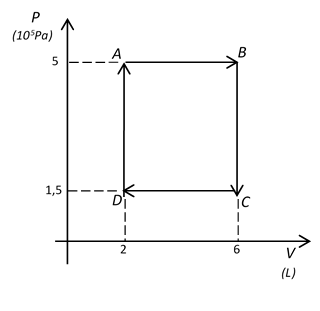
\includegraphics{./capitulo_04/termodin.png}
% \caption{Ejemplificacin de diagrama en blanco y negro.}
% \label{fig:termodin}
% \end{center}
% \end{figure}

% Las tablas deberan contener datos representativos que sinteticen informacin significativa del trabajo, evitando mostrar datos intermedios que pudieran dificultar la interpretacin del mismo.

% Cada tabla debe estar antecedida de un epgrafe que la identifique, enumere y describa brevemente.

% Cada tabla debe ser referenciada al menos una vez, a travs de su nmero, de preferencia antes de que aparezca en el documento, como en este caso (tabla \ref{tab:animales}).

% \begin{table}[H]
% \begin{center}
% \caption{Inventario de animales.}
% \label{tab:animales}
% \begin{tabular}{||l|l|r||}
% \hline
% Especie&Sexo&Cantidad\\
% \hline
% \multirow{2}{*}{palomas}&jvenes&20\\
% &adultas&18\\
% \hline
% \multirow{2}{*}{conejos}&jvenes&5\\
% &adultos&5\\
% \hline
% \multirow{2}{*}{gallinas}&jvenes&50\\
% &adultas&50\\
% \hline
% \multicolumn{2}{||c|}{Total}&148\\
% \hline
% \end{tabular}
% \end{center}
% \end{table}

% Otro ejemplo de tabla en el cual se observa el empleo de color, adems de la combinacin de columnas se observa en la tabla \ref{tab:color}

% \begin{table}[H]
% \begin{center}
% \caption{Clasificacin de la muestra, por edad.}
% \label{tab:color}
% \begin{tabular}{|c|cccc|}
% \hline
% \multirow{2}{*}{\cellcolor[rgb]{0.4,0.8,0.5}} &  \multicolumn{4}{>{\cellcolor[rgb]{0.4,0.8,0.9}}c|}{Tamao de las muestras} \\ 
% \cellcolor[rgb]{0.4,0.8,0.5}Edad&\cellcolor[rgb]{0.4,0.8,0.9} San Lorenzo &\cellcolor[rgb]{0.4,0.8,0.9} Asuncin &\cellcolor[rgb]{0.4,0.8,0.9} Villarrica &\cellcolor[rgb]{0.4,0.8,0.9} Encarnacin \\
% \hline
% e$<$20 &  93 &  74 &  68 & 87 \\
% 19$<$e$<$40 &  52 &  48 &  69 & 70 \\
% 39$<$e$<$60 &  47 &  85 &  81 & 64 \\
% 59$<$e$<$80 &  28 &  36 &  16 & 23 \\
% 79$<$e &  9 &  5 &  6 & 12 \\
% \hline 
% \end{tabular}
% \end{center}
% \end{table}

% Aveces, como en el caso de la tabla \ref{tab:color}, el cdigo se vuelve bastante complejo que resulta engorroso obtener en tiempo razonable la apariencia esperada de la tabla. En esos casos; es posible elaborar la tabla en entorno diferente a Latex; grabarla como imagen png, o jpg, o pdf; e insertarla enmascarada como tabla para ser contada como una de ellas por el contador de tablas: esto se logra con incluir la imagen dentro del entorno ``table'', como se ejemplifica con la tabla \ref{tab:tabla_word} que sigue.

% \begin{table}[H]
% 	\begin{center}
% 		\caption{Imagen de tabla, en reemplazo de la tabla anterior.}
% 		\label{tab:tabla_word}
% 		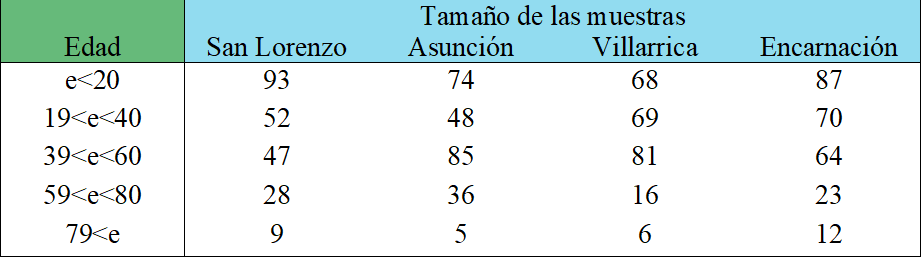
\includegraphics[scale=.65]{./capitulo_04/tabla_word.png}
% 	\end{center}
% \end{table}
\renewcommand{\labelitemi}{$-$}

